16. Write the equation of the graph presented below in the form $f(x)=ax^2+bx+c$, assuming  $a=1$ or $a=-1$. Then, choose the intervals that $a, b,$ and $c$ belong to.
\begin{center} 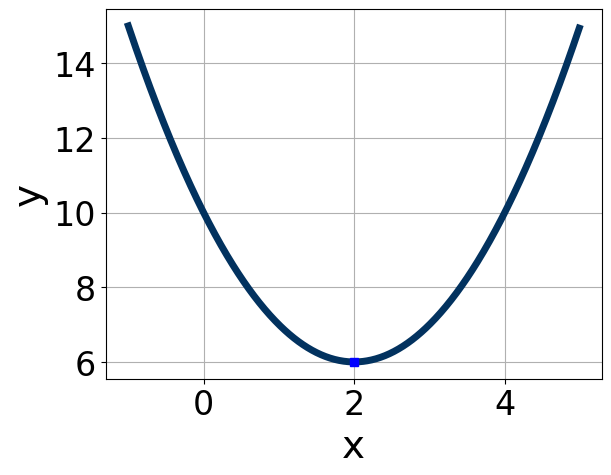
\includegraphics[scale=0.5]{../Figures/quadraticGraphToEquationA.png} \end{center}The solution is $ f(x) = -1x^{2} +4 x -10 $ 

\begin{enumerate}[label=\Alph*.] 
\item $ a \in [-1.3, 0.8], \hspace*{5mm} b \in [3, 6], \text{ and } \hspace*{5mm} c \in [1, 4] $ 

  Distractor 2: This distractor corresponds to not distributing correctly (so that c is not correct). 
\item $ a \in [-1.3, 0.8], \hspace*{5mm} b \in [3, 6], \text{ and } \hspace*{5mm} c \in [-15, -7] $ 

 * This is the correct solution 
\item $ a \in [0.4, 2.2], \hspace*{5mm} b \in [-6, -3], \text{ and } \hspace*{5mm} c \in [-15, -7] $ 

  Distractor 4: This distractor corresponds to having a and b as negative. 
\item $ a \in [-2, 0], \hspace*{5mm} b \in [-6, -3], \text{ and } \hspace*{5mm} c \in [-15, -7] $ 

  Distractor 1: This distractor corresponds to having b as negative. 
\item $ a \in [-1.3, 0.8], \hspace*{5mm} b \in [-6, -3], \text{ and } \hspace*{5mm} c \in [1, 4] $ 

  Distractor 3: This distractor corresponds to having b as negative AND not distributing correctly. 
\end{enumerate} 
 
General Comments: When the graph is pointing up, $a=1$. When the graph is pointing down, $a=-1$. Be sure to use Vertex Form: $y = a(x-h)^2+k$.

-----------------------------------------------

